\begin{document}
\hypertarget{cs-131-demo-day-fall-2021}{%
\subsubsection{CS 131 Demo Day Fall
2021}\label{cs-131-demo-day-fall-2021}}

Peyton Chen

For CS 131 Demo Day, I decided to take inspiration from HW \#8 and use
PyTorch to implement a face mask detector. I found a dataset from Kaggle
at this link:
https://www.kaggle.com/ashishjangra27/face-mask-12k-images-dataset which
contained 10,000 training images, 10,000 test images, and 800 validation
images. This dataset has been invaluable in letting me train my
convolutional neural network. Much of the scaffolding code resembled HW
\#8, however, I tailored the transforms to this specific dataset with
still normalizing 0.5 mean and 0.5 standard deviation, but opting to
resize all images to 150x150 so that the input was of a predictable size
before training and inference.

For the actual neural network, I opted for the following architecture: 1
Conv2d layer, with input channels as 3 (since all the images I pass in I
plan to be colored) and output channels as 32 with a kernel size of 3. I
then had 2 more Conv2d layers with input channels as 32 and output
channels as 32 and kernel size of 3. Application of these filters
allowed the neural network to effectively gather a map of activations,
indicating the locations and strength of what a face looks like with and
without a mask. The RELU activation function is applied after each
convolutional layer. I use MaxPool after each convolutional + RELU layer
in order to reduce the size of each feature map to summarize the
features detected in the input image. After this, I flatten the input
with a \texttt{nn.Flatten()} layer before preceding to fully-connected
layers of 512 to 100 and 100 to 1 (as we are just detecting whether
someone is wearing a mask or not). I use RELU activation function here
as well but add in a dropout layer of 0.5 between the two layers to
prevent overfitting. Then, I apply the sigmoid function as we want to
generate a probability prediction. To turn this into a label of 0 or 1,
I just apply \texttt{torch.round()}.

For the optimizer, I use the Adam optimizer because I wanted a
computationally efficient optimizer as well as an algorithm that was
appropriate for problems with noisy/sparse gradients. I left learning
rate and other options as default. As this is a binary classification
problem, I opted for a binary cross-entropy loss. I trained for 5 epochs
which resulted in 99.37\% accuracy on the test set of 10,000 images and
98.62\% accuracy on the validation set with 800 images. I then, decided
to use me as a test subject by taking an (awkward) selfie and it
correctly classified me.

Finally, I decided to take this one step forward by implementing a
program to harness the webcam of a user's computer to do live mask
detection. I used \texttt{imutils} and \texttt{cv2} in order to do this.
I also used a pre-trained model with weights for the face-detection
algorithm (deploy.prototxt with SSD.caffemodel weights). Then, I
configured the face detection with the appropriate hyperparameters and
passed in every cropped face from the face-detection model to my
pretrained CNN. The program stops when the user presses the character q
while focused on the frame of the program. One observation I had for my
model in ``real-life'' usage was that the model struggled a bit with
dimly lit images/videos. As such, I found much better accuracy when I
was in a well-lit room and my face was not in a shadow, which makes
sense.

Here's a screenshot of the live-detection program.


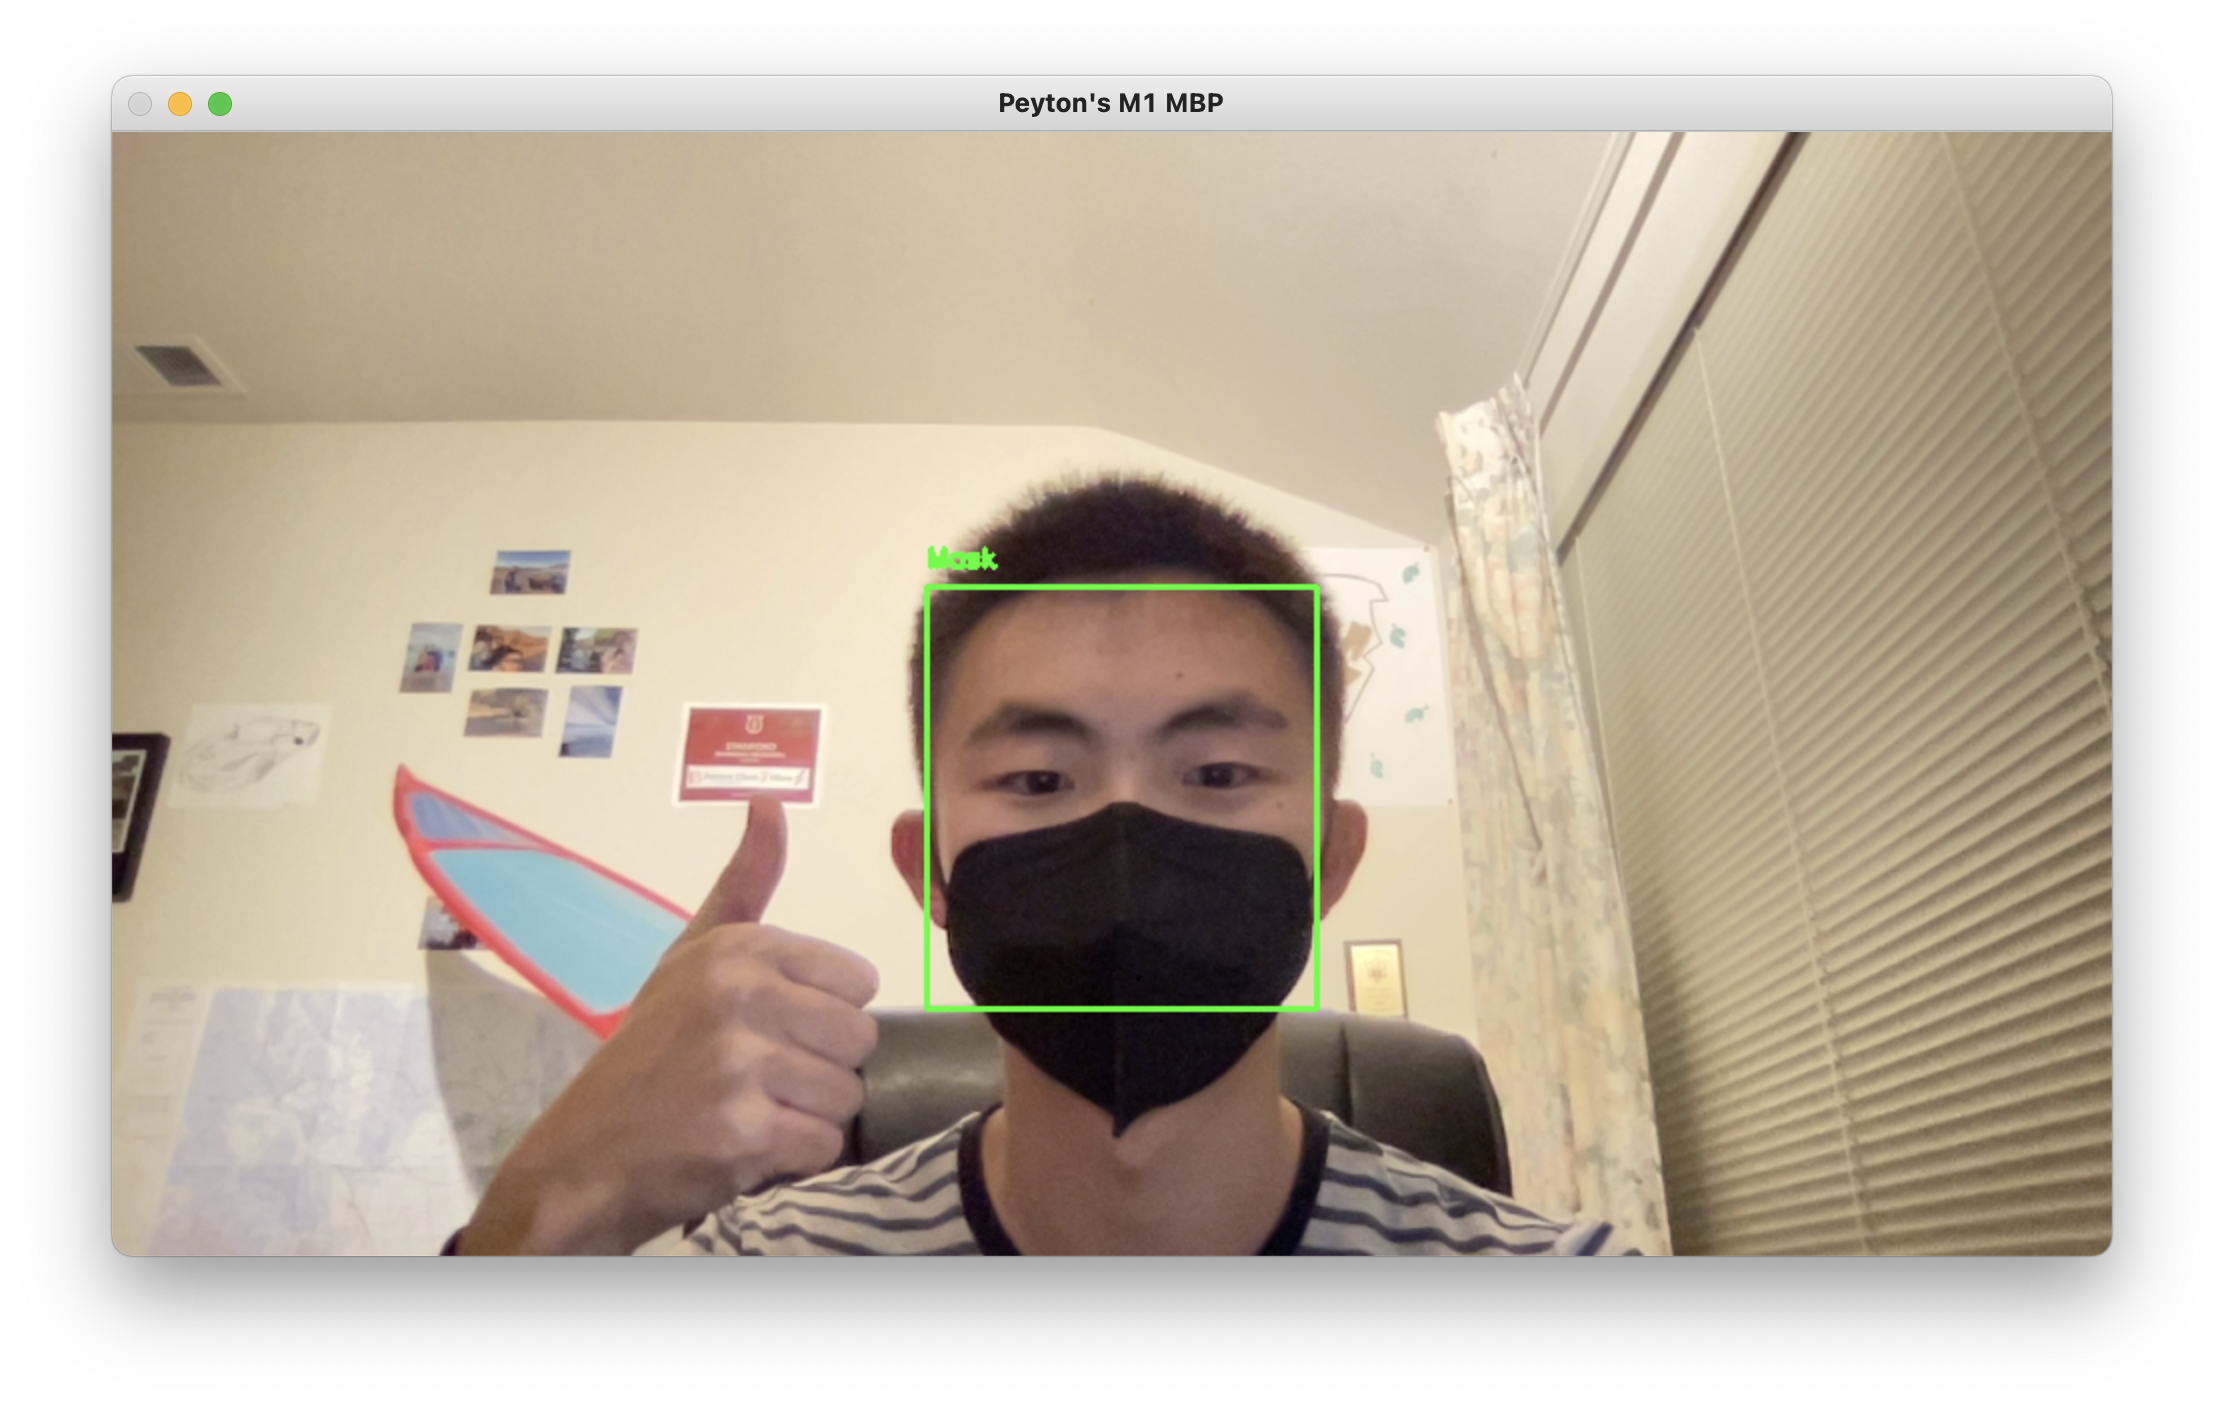
\includegraphics{live-detection.png}

To run training, look at \texttt{train.ipynb}. To run the live detection
model, use \texttt{python3\ live\_detection.py}. This project was
developed in Python 3.8.5 with PyTorch and OpenCV and miscellaneous
other dependencies in a Miniconda environment on a M1 Macbook Pro.
\end{document}